\subsection{Frequency limits and Inertia Constants}
When the global security of the system is endangered and under/above frequency is experienced, the load shedding is activated; the system is said to be in the emergency state. If the frequency exceeds the range between 47.5 and 51.5 Hz, a system blackout can hardly be avoided \cite{ENTSOE.2016}. Consequently, the system will reach the so-called blackout state and will have to be restored. Before the blackout, the system tries to recover the balance by rejecting partial load starting at 49 Hz as frequency decreases. On the other hand, curtailment thresholds between 50.2 and 50.5 Hz have been studied by ENTSOE for over-frequency scenarios \cite{ENTSOE.2016}. In this research, a deviation of $ \pm1 $ Hz is used as threshold before load shedding and curtailment starts. Hence, to keep frequency within such threshold; the investigated critical time and power response, corresponding to the maximum allowed time for fast power reserve activation. In the case of under-frequency power is injected in the system whereas, in the over-frequency case, power is extracted from the grid.

Two terms commonly found in the literature of power system stability will be used along this section:

\begin{itemize}[leftmargin=*,labelsep=5.8mm]
\item \textbf{Inertia constant (H)}: It has units of seconds (s) and it is the ratio of the stored kinetic energy in the rotating masses of the machine ($E_k$ in MWs) and its nominal capacity ($S_{nom}$ in MVA).\\
\item \textbf{Acceleration time constant (T\textsubscript{a})}: It also has the units of seconds (s) but this is the ratio of double the kinetic energy (MWs) and the generator nominal power output ($P_{nom}$ in MW).\\
Acceleration time constant is a measure of the robustness against disturbances of the system. It could be interpreted as the required time to remove the kinetic energy from the rotating masses of the generators connected in a grid at the rate of the supplied power load. Hence, the higher the time constant, the higher the kinetic energy available. As the share of synchronous generations decreases, this constant decreases proportionally.
\end{itemize}

With $f$ as frequency, $f_0$ as nominal frequency and $\Delta P$ as power imbalance, the swing equation can be expressed as follows \cite{kundur1994power}:
%Equation 3 1
\begin{equation}
\label{eq:swing}
\frac{df}{dt}=\dfrac{\Delta P*f_0}{2*H*S_{nom}}=\frac{\Delta P*f_0}{T_a*P_{nom}}=\frac{\Delta P*f_0}{2*E_k}
\end{equation}

In this paper, the inertia constant $ H $ is used for the description of inertia in wind turbines and single synchronous machine representation whereas the system acceleration constant $ T_a $ is used to express the whole system inertia related to the load in terms of real power.

\subsection{Frequency Support from Inverter based Generation}

In this section, the methodology and considerations for the implementation of inverter-based generation for frequency support are explained.

\subsubsection{Synthetic Inertia}

Synthetic inertia is one of the techniques that manufactures and researchers are considering to tackle the low inertia problem in power systems \cite{Gevorgian.2017, GeneralElectricInternational.2013}. Frequency support through synthetic inertia was considered with the following assumptions \cite{dreidy2017inertia, nesje2015need}:
\begin{enumerate}[leftmargin=*,labelsep=4.9mm]
\item Power output from synthetic inertia is limited to 10\% of the wind turbine nominal power.
\item Due to mechanical and thermal stresses, the additional power can be delivered only for a maximum time of 10 s.
\item It is assumed that all wind turbines operate at its nominal power output. The value of 1.5 MW was selected for such purpose.
\item The maximum allowable amount of kinetic energy to be extracted from the turbines was limit to half of the kinetic energy while the turbine operates at nominal speed \cite{NREL.2012}.

\end{enumerate}

A control system is needed so the stored energy in the rotating blades can be extracted from the wind turbine. Using the expression of power as the derivative of the stored energy in the blades Equation \eqref{eq:si} is obtained. The additional extracted power from the wind turbine through the implementation of Equation \eqref{eq:si} accounts for the synthetic inertia contribution \cite{NREL.2012}.

\begin{equation}
\label{eq:si}
P_{pu}(t)=2*H_{wt}*\omega_{pu}(t)*\dfrac{d\omega_{pu}(t)}{dt}
\end{equation}

%Equation 3 4

Where $H_{wt}$ is the turbine inertia constant and $\omega_{pu}$ the rotational speed in per unit.

\begin{figure}[h]
\centering
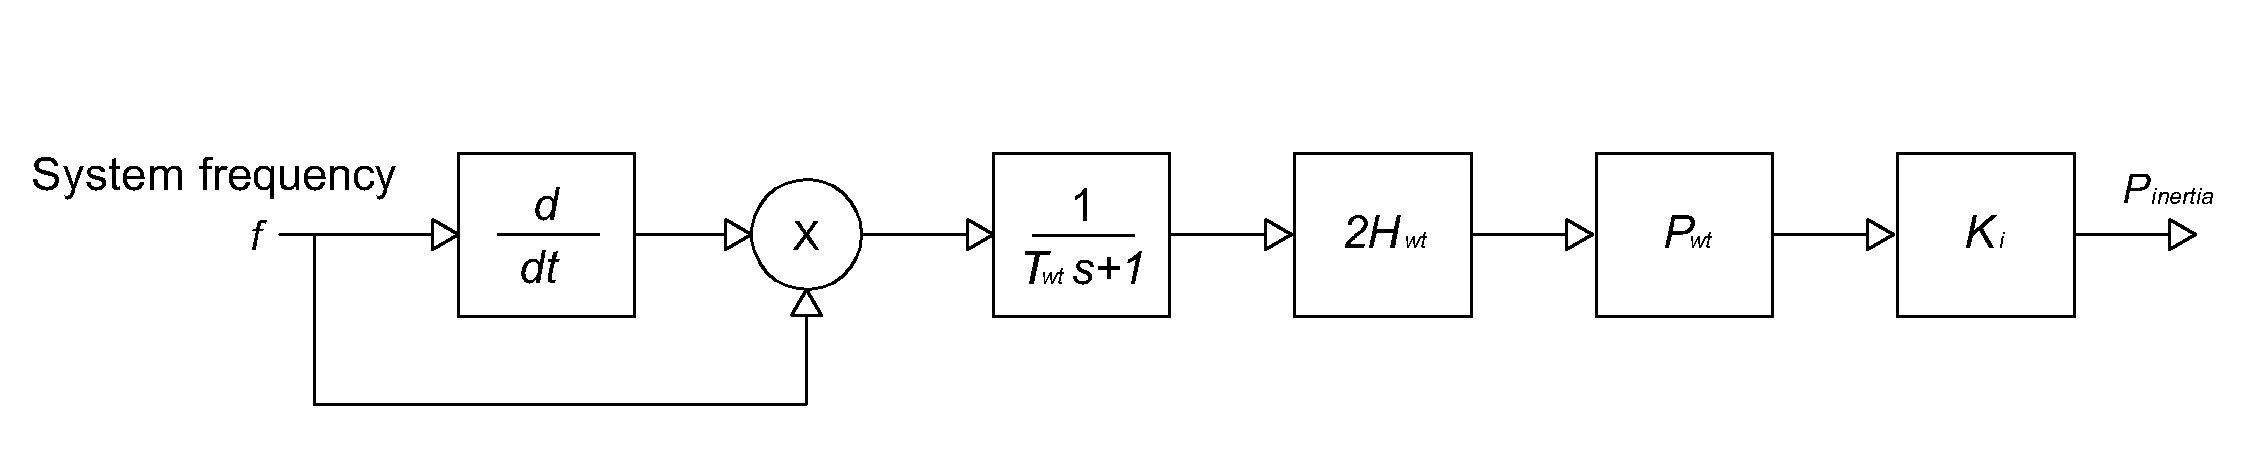
\includegraphics[width=0.8\textwidth]{/method/SI2}
\caption{Representation of Equation \eqref{eq:si} in Simulink. In the figure it can be seen the insertion of a filter at the output of the multiplication block \cite{GeneralElectricInternational.2013, nesje2015need}. A constant block $ K_i $ adjusts the initial response in the model. Since Equation \eqref{eq:si} is given in pu, the output is multiplied by a constant $ P_{wt} $ representing the rated power of the turbine.}
\label{fig:synthetic}
\end{figure}

Typical values of inertia constant for wind turbines are not openly available from the manufacturers to the public. An approximate value was calculated with the utilization of an equation which relates nominal power and inertia constant for wind turbines \cite{GonzalezRodriguez.2007}.

\begin{equation}
\label{eq:wtinertia}
H_{wt}\approx1.87*P_{nwt}^{0.0597}
\end{equation}


For a wind turbine with a nominal power output of 1.5 MW, the value of $ H $ corresponds to 4.37 s \cite{Wu.2013}. Rated rotational speed of 18 rev/min was considered \cite{Wu.2013}. To avoid the wind turbine to stall, a reduction of 5 rev/min is allowed by the implementation of the control system. This change of rotational speed equals a reduction of 3 MWs on kinetic energy out of a total of 6 MWs.

%Table 3 1: Constants for implementation of synthetic inertia.
\begin{table}[h]
\caption{\label{tb:inertia}: Constants for the implementation of synthetic inertia in Simulink, $ n_{wt} $ represents the number of wind turbines with synthetic inertia control}
\centering
%% \tablesize{} %% You can specify the fontsize here, e.g., \tablesize{\footnotesize}. If commented out \small will be used.
\begin{tabular}{cccc}
\toprule
\textbf{T\textsubscript{wt}} & \textbf{ H\textsubscript{wt} (s)}	& \textbf{ P\textsubscript{wt} (MW)} & \textbf{ K\textsubscript{i}} \\
\midrule
1 & 4.37 & 1.5*$ n_{wt} $ & 10 \\
%entry 2 & data & data\\
\bottomrule
\end{tabular}
\end{table}

\subsubsection{Inverter based fast Power Reserve}

When a power system is subjected to a negative power imbalance and it is assumed that no load is rejected at UFLS frequency, this continues dropping below 49 Hz. The time at which the system frequency equals the UFLS value is then called critical time. This is the maximum available time for the inverter based reserve to deploy the required power to the system.

\begin{figure}[h]
\centering
\begin{subfigure}[h]{0.45\textwidth}
\centering
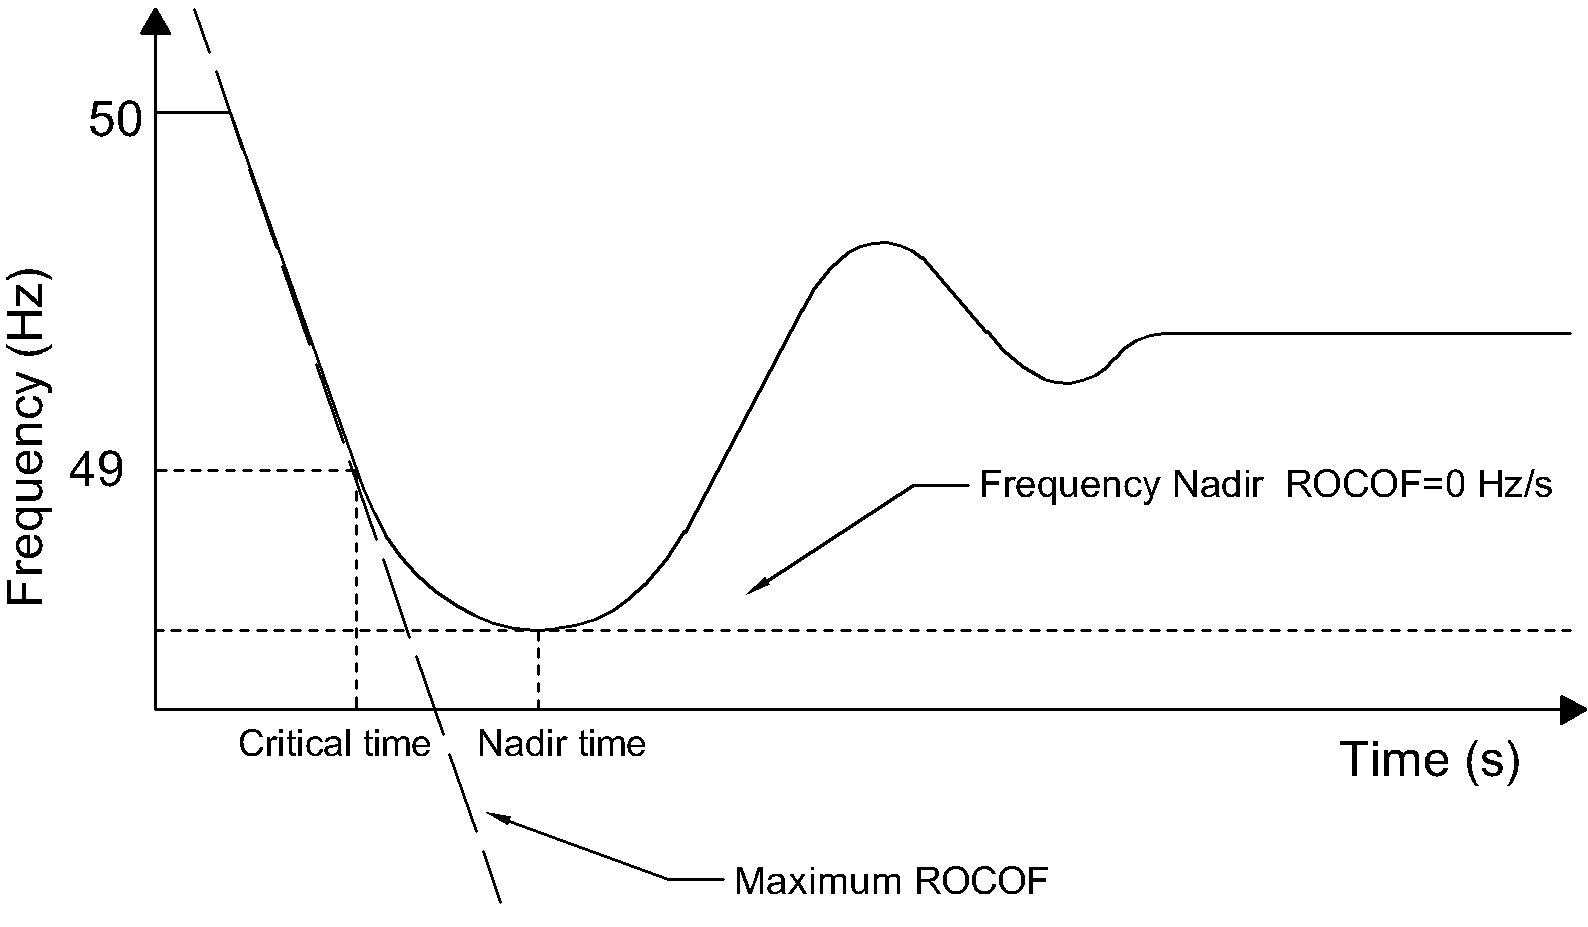
\includegraphics[width=\textwidth]{method/fig1}
\caption{Without IBFPR}
\label{fig:freqresp_before}
\end{subfigure}
\hfill
\begin{subfigure}[h]{0.45\textwidth}
\centering
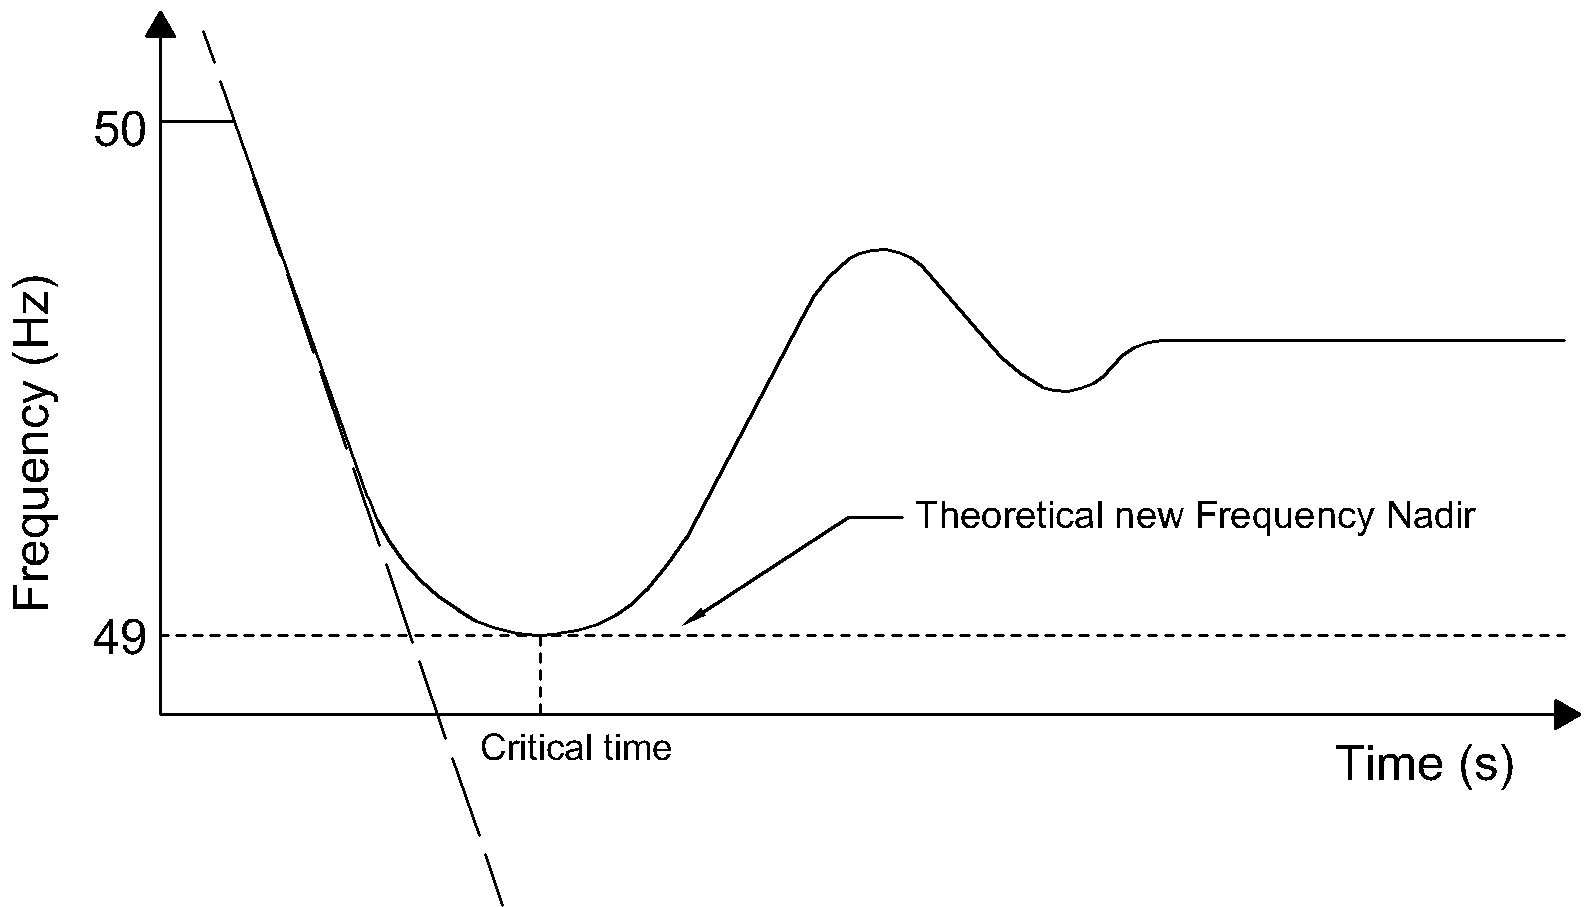
\includegraphics[width=\textwidth]{method/fig2}
\caption{With IBFPR}
\label{fig:freqresp_after}
\end{subfigure}


\caption{In (\textbf{a}) the frequency response goes below the 49 Hz leading to UFLS at the critical time, whereas in (\textbf{b}) the IBFPR is applied to avoid ULFS. In this case, the power imbalance is compensated at the critical time by the inverters.}
\end{figure}

In the critical condition that would lead to load shedding, it is expected from the IBFPR to at least counteract the RoCoF at the critical time, as illustrated in Figure \ref{fig:freqresp_after}.
Recalling Equation \eqref{eq:swing}; it is necessary that the machine accelerating power (power imbalance) become zero at the critical time.
\begin{equation}
\label{eq:powerbalance}
P_a (t_{cr} )=P_{mech}-P_{elec}+P_{IBFPR}=0
\end{equation}

Where $ P_a $ is accelerating power, $ P_{mech} $ is mechanical power, $ P_{elec} $ is electrical power load, $ t_{cr} $ is the critical time and $ P_{IBFPR} $ is inverter based fast power reserve.

From the assumption of a linear mechanical power deployment of the synchronous machines governors, the rate of change in mechanical power, after a power imbalance $ \Delta P $, is given by $ \Delta P/t_{nadir} $, where $ t_{nadir} $ represents the time at which the frequency nadir occurs. Given the power balance at the critical time, $ t_{cr} $; the IBFPR response must be equal to $ P_{elec}-P_{mech} $, being $ P_{elec} $ equal to $ \Delta P $.


Substituting $ P_{mech} $ by $ \Delta P* t_{cr} /t_{nadir} $ and $ P_{elec} $ by $ \Delta P $ in Equation \eqref{eq:powerbalance}, the following expression is obtained for the $ P_{IBFPR} $ at time $ t_{cr} $:
%Equation 3 2
%[
\begin{equation}
\label{eq:p_at_tcr}
P_{IBFPR} (t_{cr} )=\Delta P*(1-t_{cr}/t_{nadir} )
\end{equation}
It is assumed that $ P_{IBFPR} $ remains with a constant power output after $ t_{cr} $ long enough to stabilize the system frequency. The result of the previous equation represents the slope of the power output since the inception of the incident until the critical time, which with the implementation of IBFPR will be not any longer critical but rather it will be the new desired frequency nadir time.
%Equation 3 3: IBFPR before critical time.
\begin{equation}
\label{eq:IBFPR}
P_{IBFPR} (t)=\dfrac{\Delta P*(1-t_{cr}/t_{nadir} )*t}{t_{cr}}
\end{equation}

According to the obtained expression in Equation \eqref{eq:IBFPR}; it can be realized that the desired power response from the inverters depends exclusively on parameters that cannot be directly measured from the grid connecting point. In a real situation the values of $\Delta P$, $ t_{nadir} $ and $ t_{cr} $ cannot be known in advance, representing these factors a challenge in the implementation of this ideal power response. Those values are dependent on the grid characteristics, the primary conventional reserve deployment time and the overall system inertia \cite{orum2015future}. Thus, two main cases are considered for the remaining analysis with the intent of covering a wider range of systems with different characteristics and dimensions.

\subsection{Simulation Cases}

As presented in the previous section, the values of critical time and frequency nadir depend on the system imbalance and primary reserve deployment time. In spite of assessing the influence of the grid size and the primary reserve characteristics, two main cases are considered. In both cases is assumed that the initial steady frequency is the nominal 50 Hz.


\begin{itemize}[leftmargin=*,labelsep=5.8mm]
\item \textbf{Small scale grid case:} For the evaluation a well-known and studied benchmark grid topology as the WSCC model, also known as the IEEE 9 bus model, is considered. Synchronous reserve deployment is in the order of a few seconds due to governor response \cite{kundur1994power, sundaram2008comparing}. In order to assess the typical simplifications made in power system analysis, two approaches of these cases were developed:
\subitem Scenario A - Simplified Model: The power system is represented by an equivalent single machine model in which losses are neglected. In this case, typical governor data is considered. It is investigated the critical time for inverters' activation and the required IBFPR is also determined. Furthermore, the impact of synthetic inertia is analyzed.
\subitem Scenario B - Extended Model: All the power system components (transmission lines, transformers, exciters and governors of the three generators) and its dynamic characteristics are considered in the IEEE 9 bus model for critical time and IBFPR estimation.\\
\item \textbf{Large scale grid case:} The European grid-scale in which all the synchronous machines are modeled and simplified as one single machine, provided with the characteristic expected from the overall system. Synchronous primary reserve deployment is in the order of $ \sim30 $ s \cite{ENTSOE.2016, hultholm2015optimal}. The frequency response is assumed to be the same that the European response analyzed by ENTSOE \cite{ENTSOE.2016}. Similarly, as in the simplified model of the IEEE benchmark, the influence of synthetic inertia and IBFPR is evaluated.
\end{itemize}

\begin{table}[h]
\caption{\label{tb:summary}: Summary of the simulated cases}
\centering
%% \tablesize{} %% You can specify the fontsize here, e.g., \tablesize{\footnotesize}. If commented out \small will be used.
\begin{tabular}{lcc}
\toprule
\textbf{Cases}	& \multicolumn{2}{c}{\textbf{Assessment}} \\

\midrule
{}&IBFPR&	Synthetic Inertia\\
\midrule
Small scale grid &{} &{}\\
{	a) Simplified IEEE model}	& X &	X\\
{	b) Extended IEEE model}&	X &{}\\
Large scale grid&	X&	X\\
\bottomrule
\end{tabular}
\end{table}
Therefore with the selected cases, the critical and nadir time are estimated through the simulation of different scenarios combining a range of imbalances and shares of non-synchronous generation. In order to assess Equation \eqref{eq:IBFPR}, a fit of the critical time as function of RoCoF is carried out. With the corresponding fit function for each case, Equation \eqref{eq:IBFPR} can be easily applied assuming that the inertia of the system is known and power imbalance can be calculated as: $ \frac{df}{dt}\frac{T_aP_{LOAD}}{f_0} $.

%\begin{equation}
%\Delta P(t)=\dfrac{df}{dt}\dfrac{T_aP_{LOAD}}{f_0}
%\end{equation}

%\begin{figure}[h]
%	\centering
%	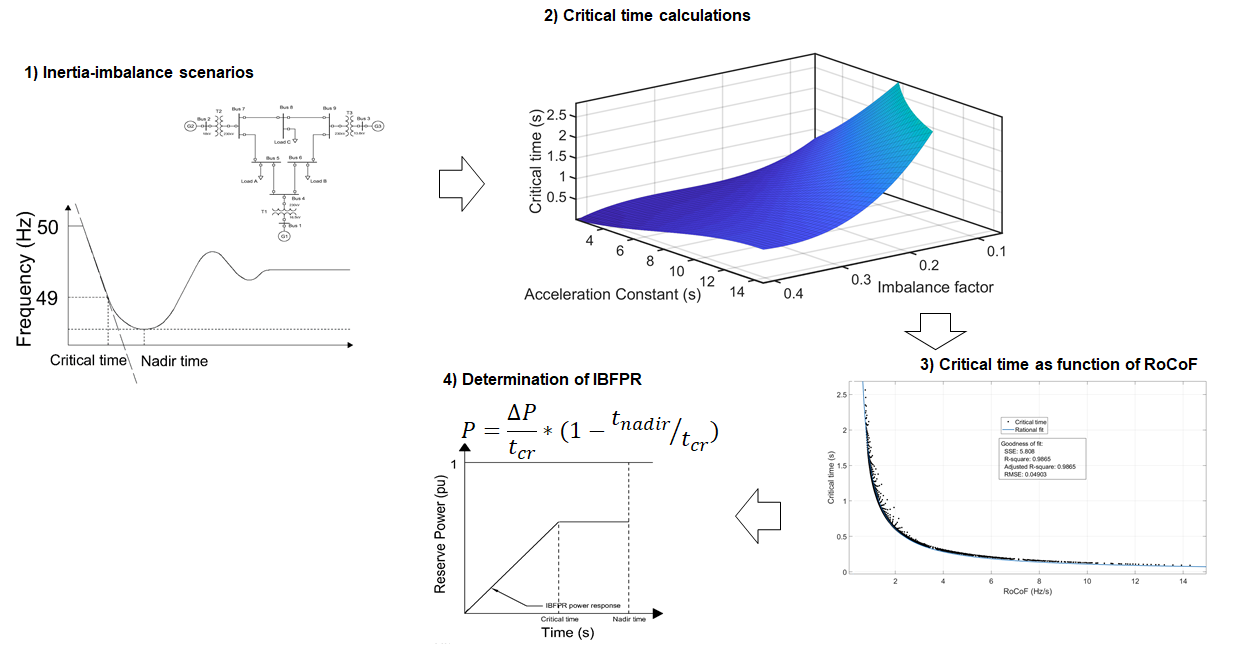
\includegraphics[width=0.6\textwidth]{/method/method}
%	\caption{IBFPR methodology: \textbf{1}) Scenarios with different system's inertia and power imbalance are simulated \textbf{2}) Critical time and nadir time is obtained for each scenario \textbf{3}) A fit function relating critical time and RoCoF is obtained \textbf{4}) According to the RoCoF measured in the system, a power response is calculated and injected to the system.}
%	\label{fig:method}
%\end{figure}


\subsection{Simplified IEEE 9 bus Model}
\label{ssec:simpleieee}

As a first step to evaluate the impact of inverter-based generation and power imbalances in the grid, the whole system is simplified as one single generating unit; neglecting all losses in the system (Transformers, transmission lines and generators) with the assumption that the mechanical output of the prime mover is the same than the electrical power output at generator terminals. Table \ref{tb:gridelements} provides a summary of the elements comprising the base model.\\




\begin{table}[h]
\caption{\label{tb:gridelements}: Elements of the IEEE 9 bus model.}
\centering
%% \tablesize{} %% You can specify the fontsize here, e.g., \tablesize{\footnotesize}. If commented out \small will be used.
\begin{tabular}{ccc}
\toprule
\textbf{}	& \textbf{Quantity}\\
\midrule
Buses & 9 \\
Transformers & 3 \\
Transmission Lines & 6 \\
Generators & 3 \\
Load & 315 MW \\
\bottomrule
\end{tabular}
\end{table}





Figure \ref{fig:ieeesimple} is the block representation of the swing equation \eqref{eq:swing}, it only differs in the fact that blocks representing the inverter-based generation have been included. The mechanical power is represented by the output of a steam turbine governor model, which is used to represent the synchronous machine as depicted in Figure \ref{fig:gov}. When equilibrium is lost, the accelerating power is multiplied by the transfer function $ 1/(2HS) $, where $ H $ is the machine’s inertia constant and $ S $ is the machine’s power rating. From Equation \eqref{eq:swing} this product equals the derivative of frequency, therefore an integrator block is added to obtain the frequency response \cite{kundur1994power, john1994power, ogata1999ingenieria}. A feedback loop is added and an error signal obtained from the reference frequency so the synchronous machine can react as frequency deviates from nominal.

\begin{figure}[h]
\centering
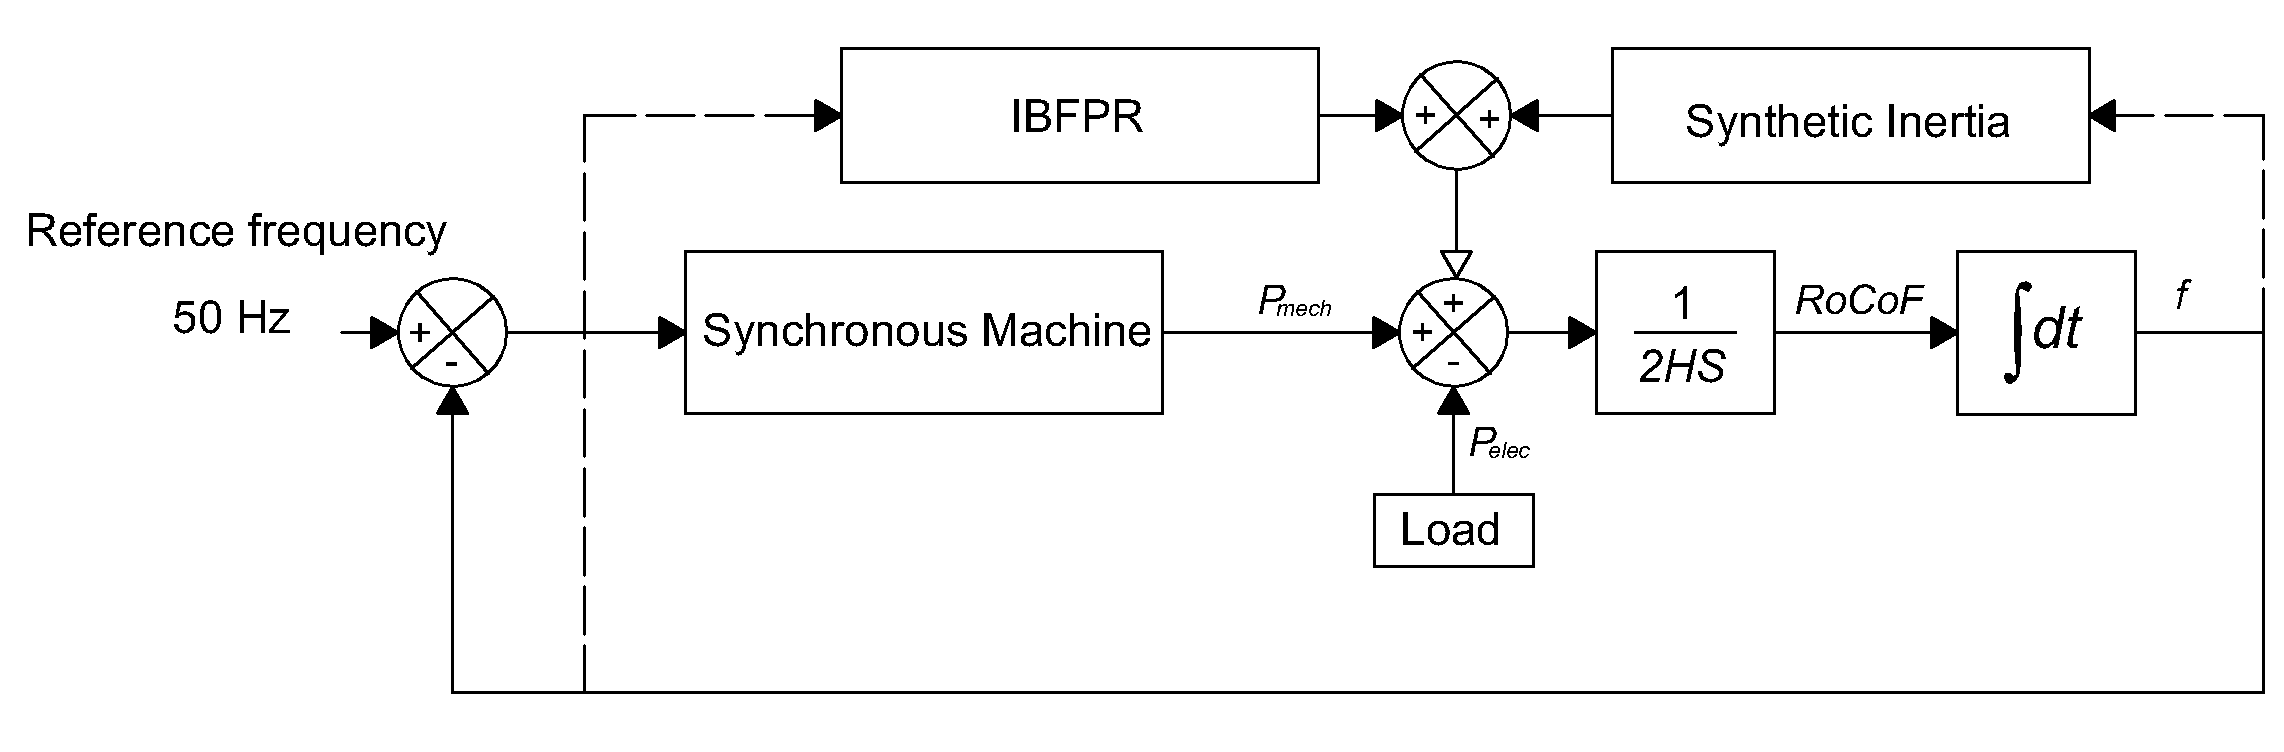
\includegraphics[width=0.75\textwidth]{/method/ieee2}
\caption{Simplified representation of the IEEE 9 bus model. Blocks linked by the solid line represent the conventional swing equation given by Equation \eqref{eq:swing}. Represented with dashed lines the respective frequency signals to the blocks of IBFPR and synthetic inertia, which add power to the system.}
\label{fig:ieeesimple}
\end{figure}


The values of kinetic energy and time constants of a synchronous machine of 835 MVA were selected to represent the synchronous response, with the load of 315 MW the system acceleration time constant is 14 s, which is approximately today’s Europe acceleration constant \cite{ENTSOE.2016}. This is the base scenario where a 100\% synchronous generation is assumed. For the sake of evaluating the impact of the penetration of inverter-based generation; the values of lower capacity generators were selected, diminishing the total system inertia.\\
\begin{figure}[h]
\centering
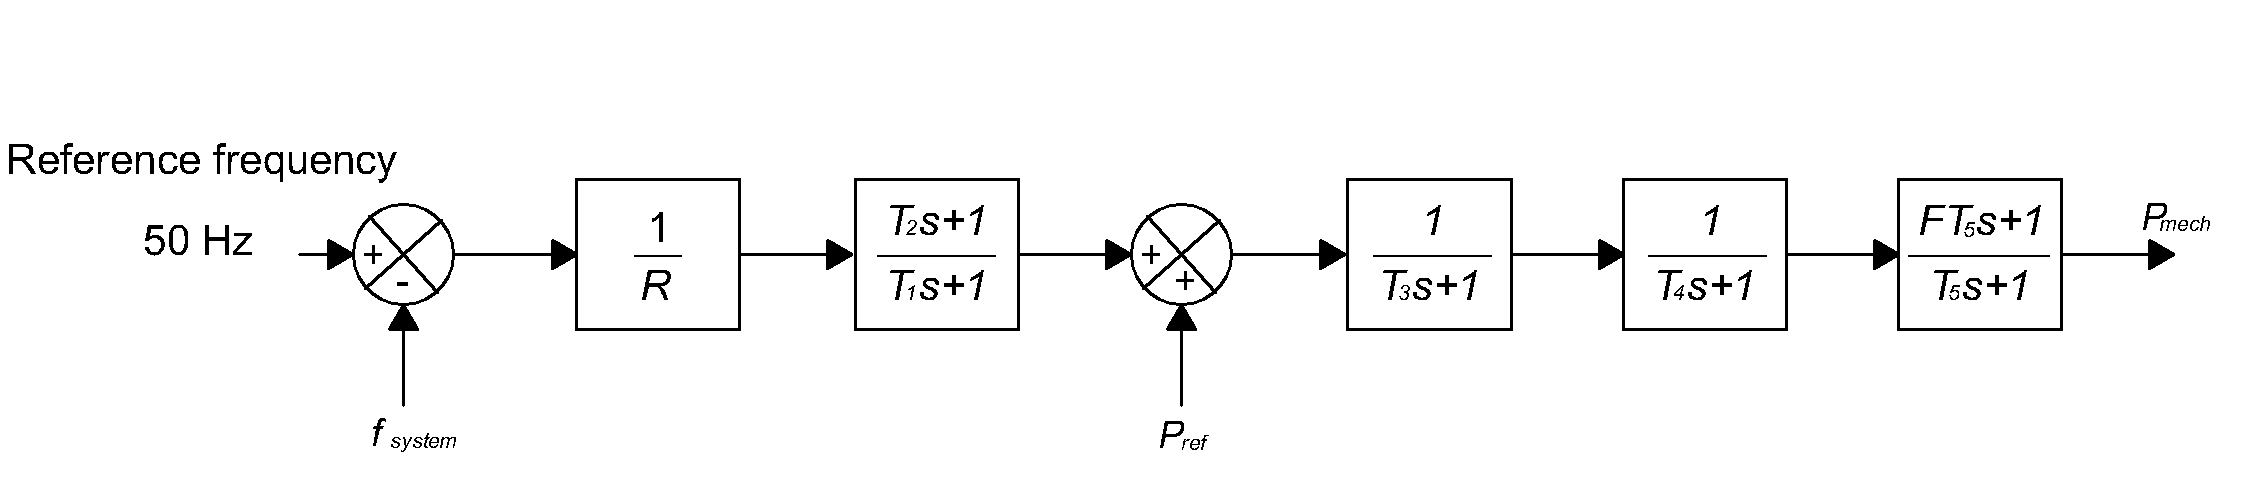
\includegraphics[width=0.75\textwidth]{/method/gov}
\caption{Model of the general-purpose governor for the representation of synchronous machines; where R is the turbine droop, P\textsubscript{ref} is the reference load at nominal frequency, T\textsubscript{1} is the governor delay, T\textsubscript{2} is the reset time constant, T\textsubscript{3} is the servo time constant, T\textsubscript{4} is the steam valve time constant and T\textsubscript{5} is the steam re-heat time constant \cite{Anderson.2002}.}
\label{fig:gov}
\end{figure}

\begin{table}[h]
\caption{\label{tb:timeconstant}: Typical generator values and governor settings as function of capacity \cite{Anderson.2002}}
%\centering
\begin{adjustbox}{width=\textwidth, center}

%% \tablesize{} %% You can specify the fontsize here, e.g., \tablesize{\footnotesize}. If commented out \small will be used.
\begin{tabular}{cccccccccccc}
\toprule
\textbf{Parameters}	& \multicolumn{11}{c}{\textbf{Generator Capacity (MVA)}} \\

\midrule
{} & 911&	835&	590&	410&	384&	192&	100&	75&	51.2&	35.29&	25 \\
\midrule

\textbf{T\textsubscript{1} (s)}&	0.1&	0.18&	0.08&	0.18&	0.22&	0.083&	0.09&	0.09&	0.2&	0.2&	0.2\\
\textbf{T\textsubscript{2} (s)}&	0&	0.03&	0&	0&	0&	0&	0&	0&	0&	0&	0\\
\textbf{T\textsubscript{3} (s)}&	0.2&	0.2&	0.15&	0.04&	0.2&	0.2&	0.2&	0.2&	0.3&	0.3&	0.3\\
\textbf{T\textsubscript{4} (s)}&	0.1&	0&	0.05&	0.25&	0.25&	0.05&	0.3&	0.3&	0.09&	0.2&	0.09\\
\textbf{T\textsubscript{5} (s)}&	8.72&	8&	10&	8&	8&	8&	0&	0&	0&	0&	0\\
\textbf{Kinetic Energy (MWs)}&	2265&	2206.4&	1368&	1518.7&	1006.5&	634	&498.5&	464&	260&	154.9&	125.4\\
\textbf{H (s)}&	2.486&	2.642&	2.319&	3.704&	2.621&	3.302&	4.985&	6.187&	5.078&	4.389&	5.016\\
\textbf{P\textsubscript{max} (MW)}&	820&	766.29&	553&	367&	360&	175&	105&	75&	53&	36.1&	22.5\\
\textbf{T\textsubscript{a} (s)}&	14.381&	14.009&	8.686&	9.643&	6.390&	4.025&	3.165&	2.946&	1.651&	0.983&	0.796\\
\bottomrule
\end{tabular}
\end{adjustbox}
\end{table}






Even though load imbalances up to 40\% were simulated in each inertia scenario, for estimation of the critical time the power capacity limit of the generators was disregarded. The negative imbalance was simulated by increasing the system load.

\subsection{Extended IEEE 9 bus Model}

Since it is desired to compare the results obtained in Section \ref{ssec:simpleieee} against some model that takes into account the whole system components, losses, and dynamics; an extended representation of the IEEE 9 bus model was implemented in Simulink \cite{delavari2018simscape}. In this representation, simulations for different values of system inertia and load imbalance were performed, similarly as it was done with the simplified representation of the model. Figure \ref{fig:ieeeext} shows the extended IEEE 9 bus grid architecture with IBG added.\\
\begin{figure}[h]
\centering
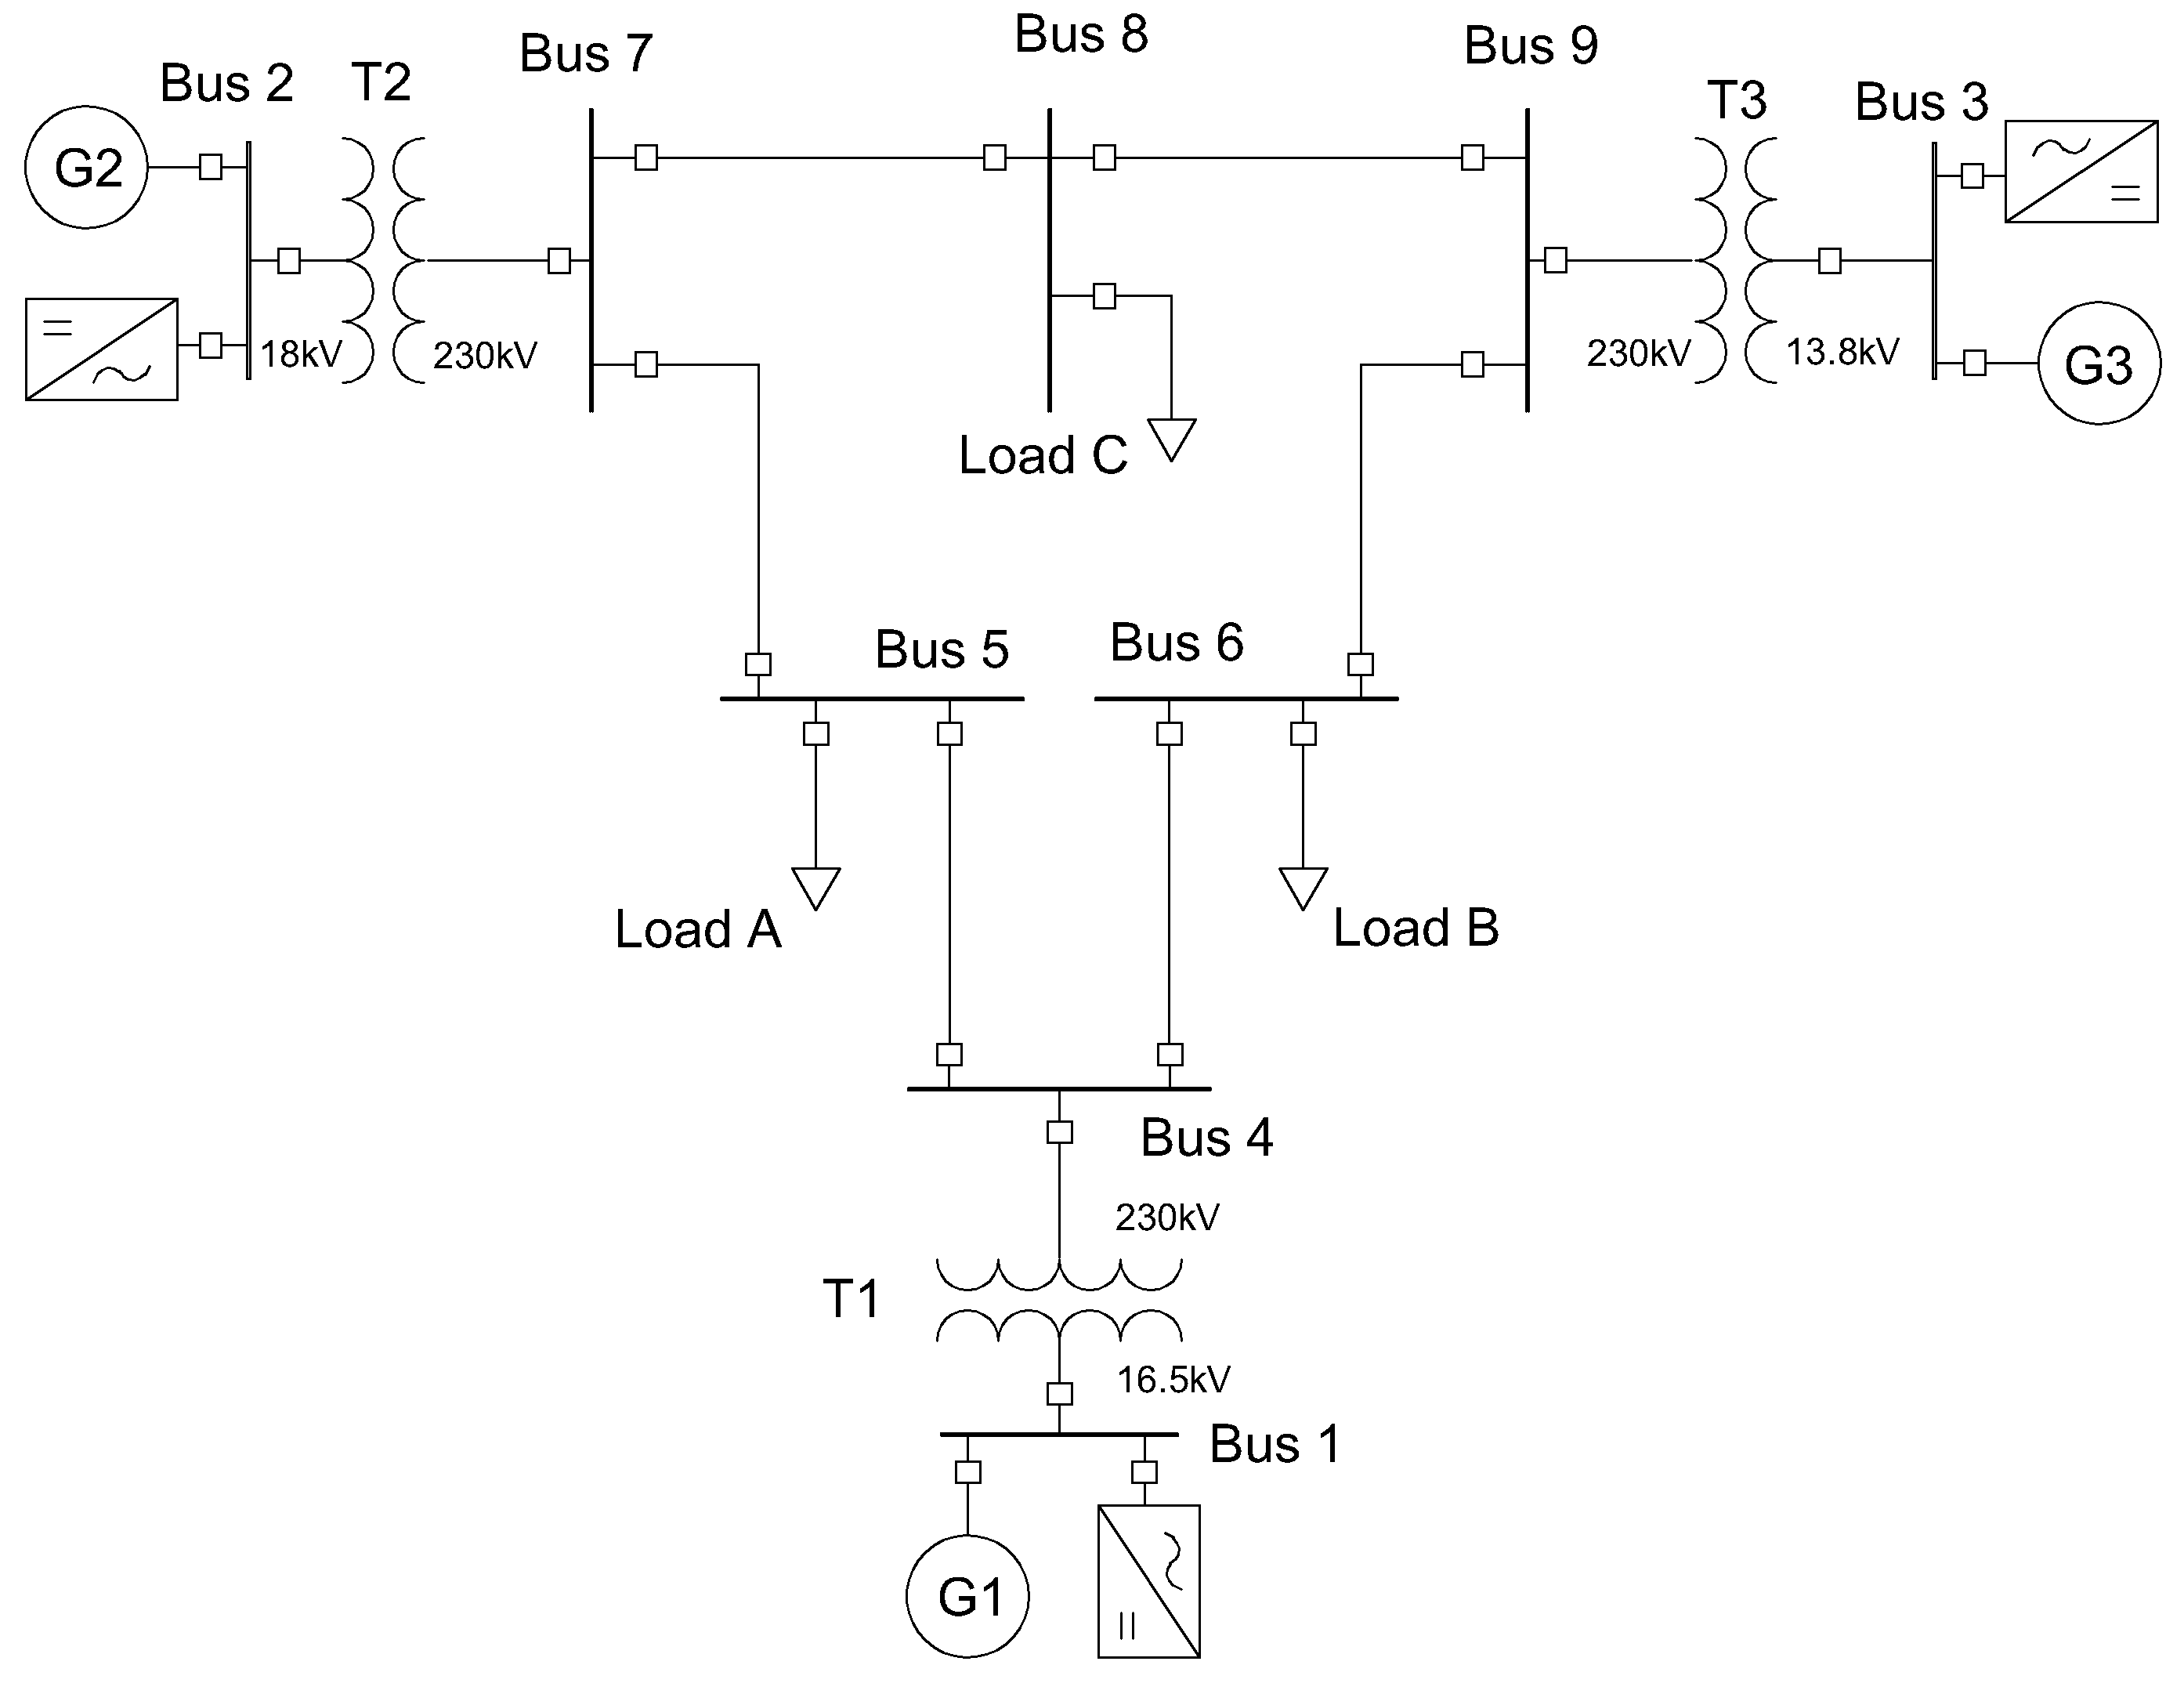
\includegraphics[width=0.5\textwidth]{/method/IEEE_FPRmodel}
\caption{One line diagram of the IEEE 9 bus model. The inverter-based frequency response has been added at the same bus of the generating units.}
\label{fig:ieeeext}
\end{figure}
In order to evaluate the validity of the equation describing the IBFPR needed to avoid ULFS, the IEEE model was modified with the insertion of ideal controlled power sources blocks, which were set up to inject power into the grid accordingly to the simulated scenario. Therefore, no means of frequency measurement were included and only IBFPR was assessed.
As it was done in Section \ref{ssec:simpleieee}, the total acceleration time constant of the system equals 14 s when there is no share of non-synchronous generation. Hence the same kinetic energy should be distributed among the three generators' rotating masses in the extended model as in the simplified representation. From Equation \eqref{eq:t_sys} it can be easily calculated that the system's kinetic energy with 14 s of acceleration time constant is 2205 MWs.
\begin{equation}
\label{eq:t_sys}
T_{sys}=2*E_{k} /P_{load}
\end{equation}

Due to the fact that inverter-based generation reduces the system kinetic energy; for different levels of inverter-based generation, the nominal capacity of the generators' values were kept constant and the inertia constant of each machine multiplied by the synchronous share factor $ fss $. The total kinetic energy of the system is the summation of all units.\\
%Equation 3 7
%E_k=2*(H*f_ss)*S
In order to start the simulations in steady-state, a load flow calculation of the grid was carried out with the objective of calculating the initial conditions for the exciter and prime mover models.
Table \ref{tb:initial} summarizes the main values for setting the system initial conditions; acquired from the power flow tool provided by SIMSCAPE.


\begin{table}[h]
\caption{\label{tb:initial}: Steady state initial conditions of the system}
\centering
%% \tablesize{} %% You can specify the fontsize here, e.g., \tablesize{\footnotesize}. If commented out \small will be used.
\begin{tabular}{ccccc}
\toprule
\textbf{Bus number}	& \textbf{Bus Type}	& \textbf{Voltage (pu)}& \textbf{Active Power (MW)}& \textbf{Reactive Power (MVAr)}\\
\midrule
1 & Slack & 1.04 $\phase{0^{\circ}} $ & 72.2 & 25.64 \\
2 & PV & 1.025 $\phase{9.83^{\circ}} $ & 163 & 8 \\
3 & PV & 1.025 $\phase{4.63^{\circ}} $ & 85 & -9.41 \\
5 & PQ & 0.9949 $\phase{-4.42^{\circ}} $ &125 & 50 \\
6 & PQ & 1.01211 $\phase{-4.16^{\circ}} $ & 90 & 30 \\
8 & PQ & 1.0172 $ \phase{0.17^{\circ}} $ & 100 & 35 \\

\bottomrule
\end{tabular}
\end{table}


\subsubsection{IBFPR Representation}


The IBFPR was modeled as controlled current sources. These controlled sources inject active power according to the load imbalance and system inertia simulated. The continuous measurement of voltage is required in order to determine the amount of current needed to supply the requested power. The IBFPR will have symmetrical and balanced characteristics. Due to this reason, the magnitude and angle of the current phasor will be obtained from the positive sequence of the measured voltage. From the definition of complex power and voltage symmetrical components in three-phase systems \eqref{eq:complex_p}, the positive sequence components of phase voltage and line current are obtained \cite{john1994power}.

\begin{equation}
\label{eq:complex_p}
S_{3\varphi}^1=3*V_{LN}^1*\bar{I}_{L}^1
\end{equation}

This equation is valid for RMS values of voltage and current in which $ S_{3\varphi}^1 $ is the positive sequence of the three-phase complex power, $ V_{LN}^1 $ is the positive sequence of voltage line to neutral and $ \bar I_{L}^1 $ is the conjugated of the positive sequence line current. Nevertheless, the measured voltage values in Simulink are peak voltages, then the equation for power and current become:

\begin{equation}
\label{eq:power_seq}
S_{3\varphi}^1=\dfrac{3*V_{LNpeak}^1*{\bar I_{Lpeak}}^1}{2}
\end{equation}


\begin{equation}
\label{eq:current_seq}
I_{Lpeak}^1=\dfrac{2*\bar{S}_{3\varphi}^1}{3*V_{LNpeak}^1}
\end{equation}
%Equation 3 10
%〖I_Lpeak〗^1=¯(((2*〖S_3ⱷ〗^1)/(3*〖V_LNpeak〗^1 )))
With the help of the \textbf{a} operator ($-0.5+j\sqrt{3}$ or $ 1\phase{120^{\circ}}) $ the values of the positive sequence component of phase voltage can be obtained. \\
From $ V_a +V_b+V_c=0$ and $ V_a^1=\frac{V_a+ aV_b+a^2 V_c}{3} $:
\begin{align*}
V_a^1 & =\dfrac{V_a+ aV_b-a^2 V_b-a^2V_a}{3} \\
& =\dfrac{V_a*(1-a^2)+ aV_b*(1-a)}{3}
\end{align*}

Since $V_{an}^1=\frac{V_a^1}{\sqrt{3}\phase{30^{\circ}}}$, $\sqrt{3}\phase{30^{\circ}}=1-a^2 $ and $ \sqrt{3}\phase{-30^{\circ}}=1-a $ then after some algebraic manipulation the expression for $ V_{an}^1 $ becomes:

\begin{equation}
\label{eq:volt_seq}
V_{an}^1=\dfrac{V_a-a^2 V_b}{3}
\end{equation}

With the obtained expressions for the positive sequence of phase voltage \eqref{eq:volt_seq} and complex power \eqref{eq:power_seq}, the needed current \eqref{eq:current_seq} to supply the IBFPR related to the measured voltages can be implemented in Simulink as depicted in Figure \ref{fig:ieeeext_ibfpr}. The ramping function will last until the critical time is reached, afterward, the IBFPR output will remain constant.

\begin{figure}[h]
\centering
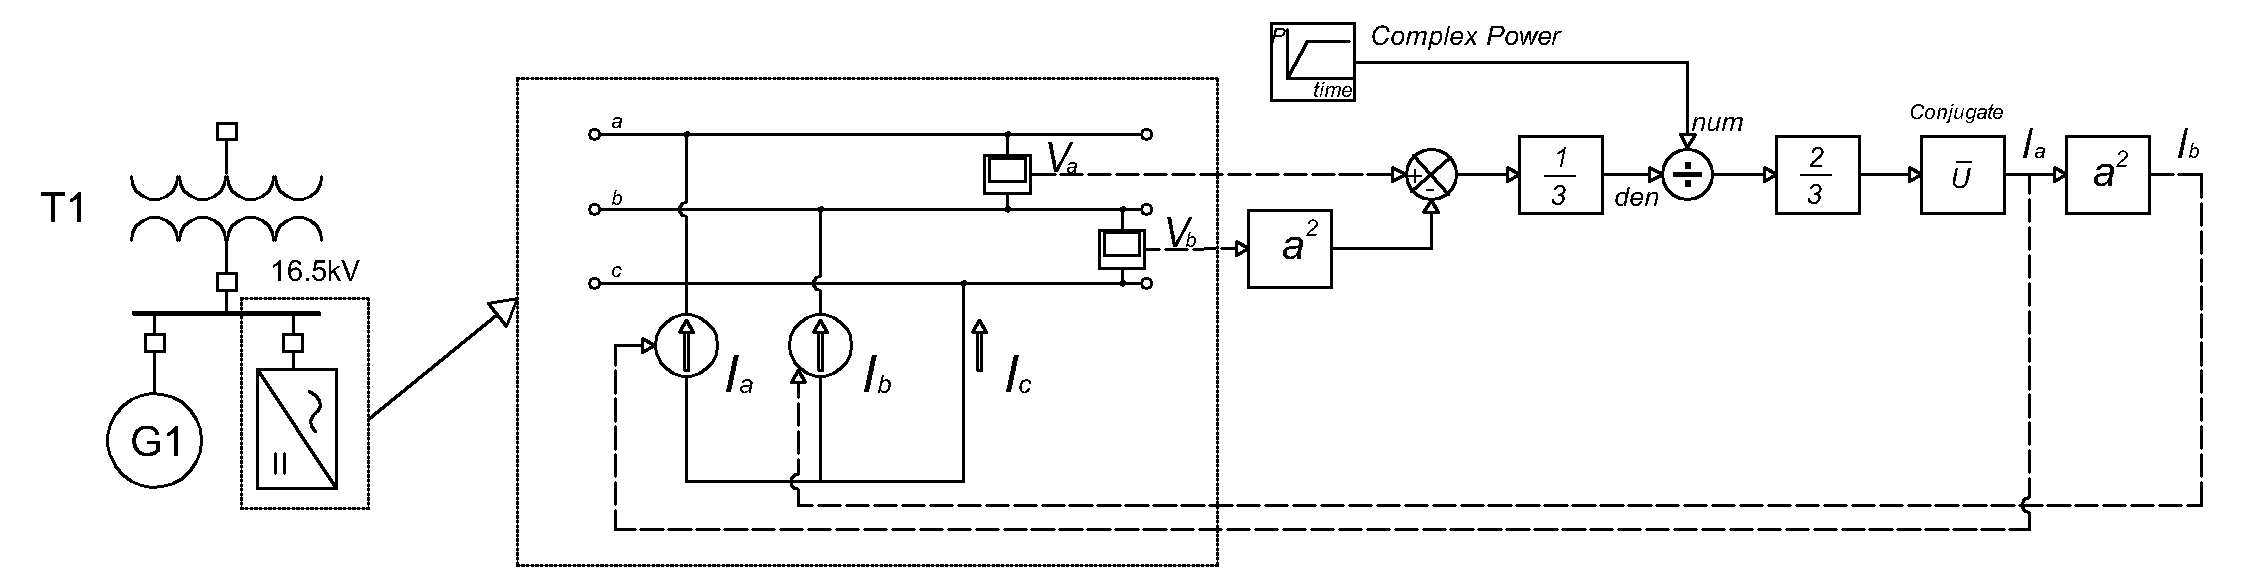
\includegraphics[width=0.75\textwidth]{/method/extended_ibfpr}
\caption{Implementation of IBFPR in the extended IEEE model. The dashed lines denote the interaction between signals from the power circuit to the control circuit and vice-versa. From the voltages readings of lines a-b and b-c the voltage $ V_{an} $ is calculated using Equation \eqref{eq:volt_seq}, then Equation \eqref{eq:current_seq} is implemented to calculate the current to be fed into the system using the complex power response obtained using Equation \eqref{eq:IBFPR} and the previous calculated value of $ V_{an} $.}
\label{fig:ieeeext_ibfpr}
\end{figure}

It must be noticed that when the IBFPR depicted in Figure \ref{fig:ieeeext_ibfpr} was implemented in Simulink, additional blocks were added in order to run the simulation, such blocks are a break algebraic loop just before the conjugate block. Additionally, a block to avoid division by zero was added at the output of the gain of $ 1 /3 $.

\subsection{Large Scale Case: Europe Power System}

Under normal operation, ENTSOE has reported values of RoCoF in the range of 5-10 mHz/s for power outages of 1 GW in the current interconnected power system. If an imbalance event of more than 3 GW occurs with depleted primary reserve, extraordinary values of frequency and RoCoF might be reached. After serious disturbances, the Continental European Power System has experienced RoCoF between 100 mHz/s and 1 Hz/s. Imbalances of 20\% or more along with RoCoF greater than 1 Hz/s have been determined by experience to be critical \cite{ENTSOE.2016}. ENTSOE has determined that the reference scenario ( loss of 3 GW generation with 150 GW load and 2\%/Hz self-regulation) in the interconnected operation, the influence of inverter-based generation, and therefore, the reduction of system inertia would not jeopardize system stability. Due to the expected increase of non-synchronous generation in the future, international power trade and renewables variability; ENTSOE estates in its future split reference scenario that the power system must be capable of withstanding imbalances greater than 40\% with RoCoF of 2 Hz/s or higher. Under these circumstances, the resulting islands must avoid load shedding. Hence, the conditions of the split scenario are considered for further analysis.
\begin{figure}[h]
\centering
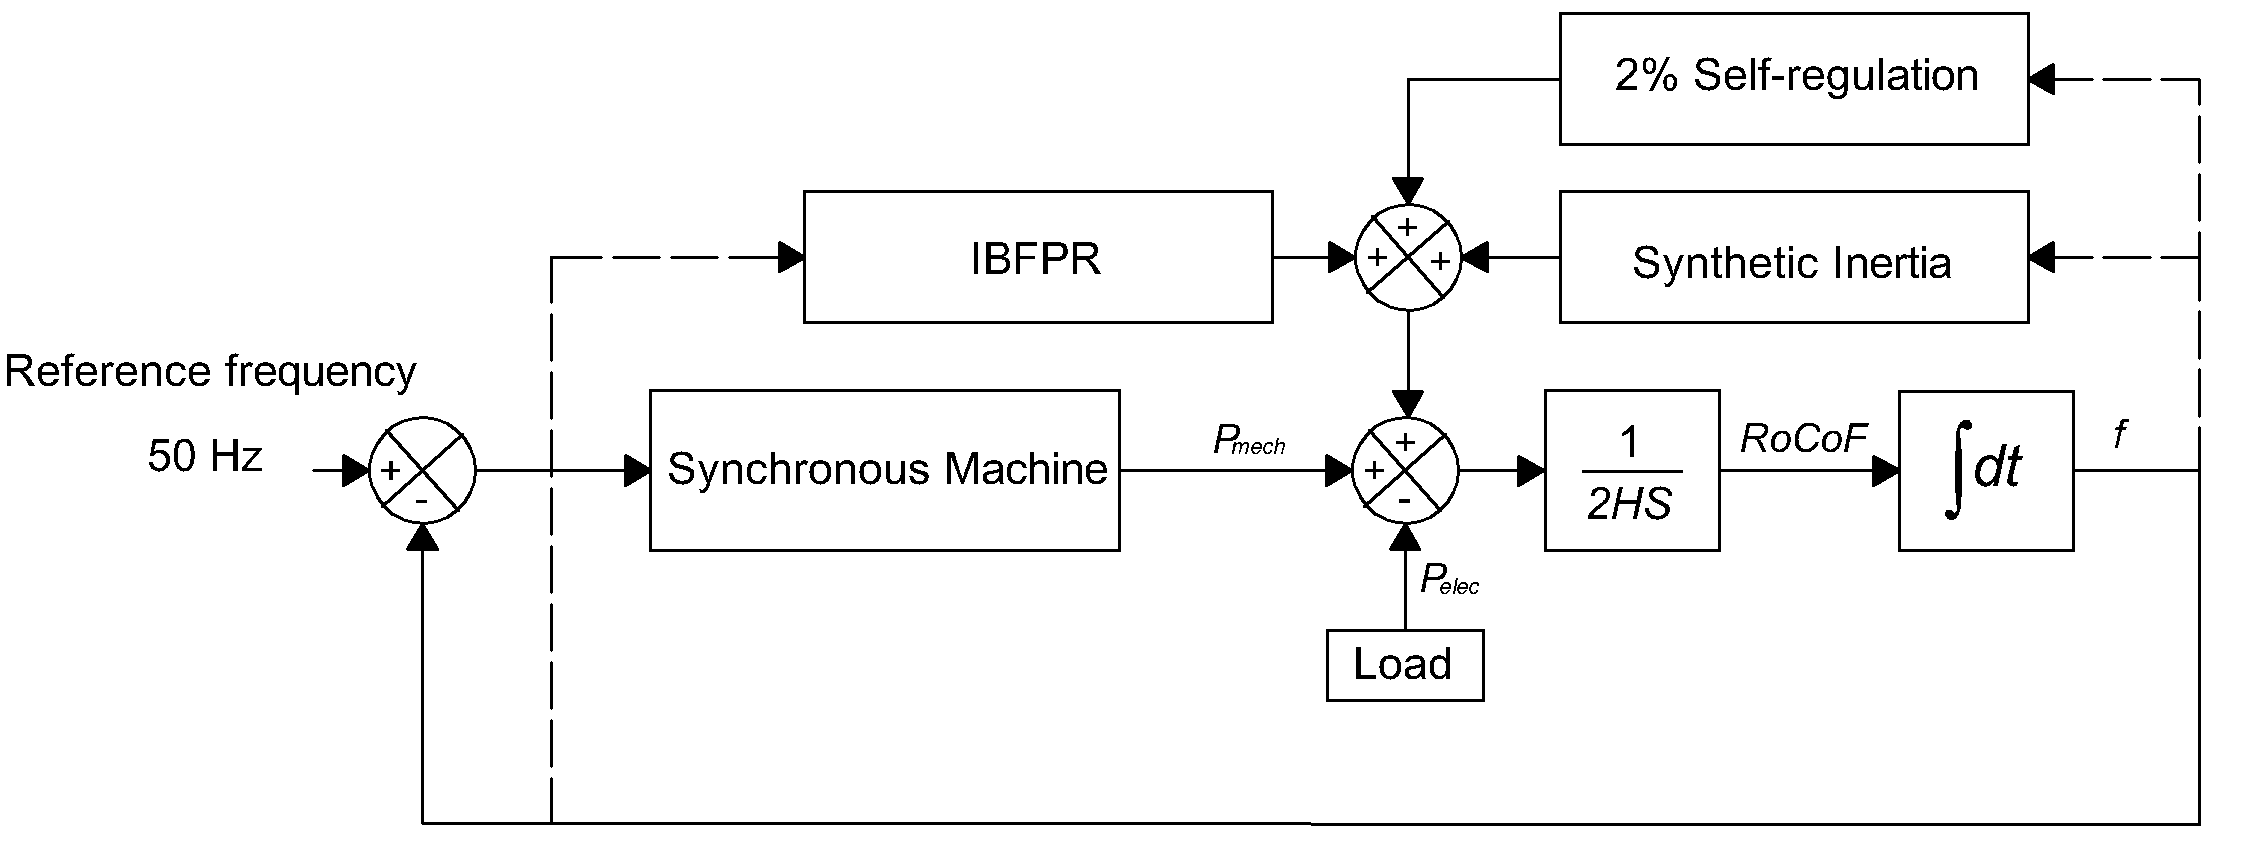
\includegraphics[width=0.6\textwidth]{/method/euro}
\caption{Large scale grid derived from the simplified IEEE model. The synchronous response was modified to match the European reserve response and the effect of self-regulation was added.}
\label{fig:euro}
\end{figure}

In order to fit the behavior of the system to the one modeled by ENTSOE, the synchronous representation in the simplified IEEE model shown in Figure \ref{fig:gov} was used as a base to emulate such behavior; this was done with the insertion of an additional block at the output of the governor model. With this approach, the primary power reserve can be easily tuned with the assistance of the Control System Tuner App available in MATLAB. The period of time of utmost interest for analysis is from the inception of the power imbalance until the nadir time. Therefore, the system must perform as similar as possible in this region compared to the ENTSOE reference, whereas after the nadir time, the disparity between responses can be neglected. On the European scale, the reserves must be completely deployed within 30 s after the occurrence of the disturbance.

\begin{figure}[h]
\centering
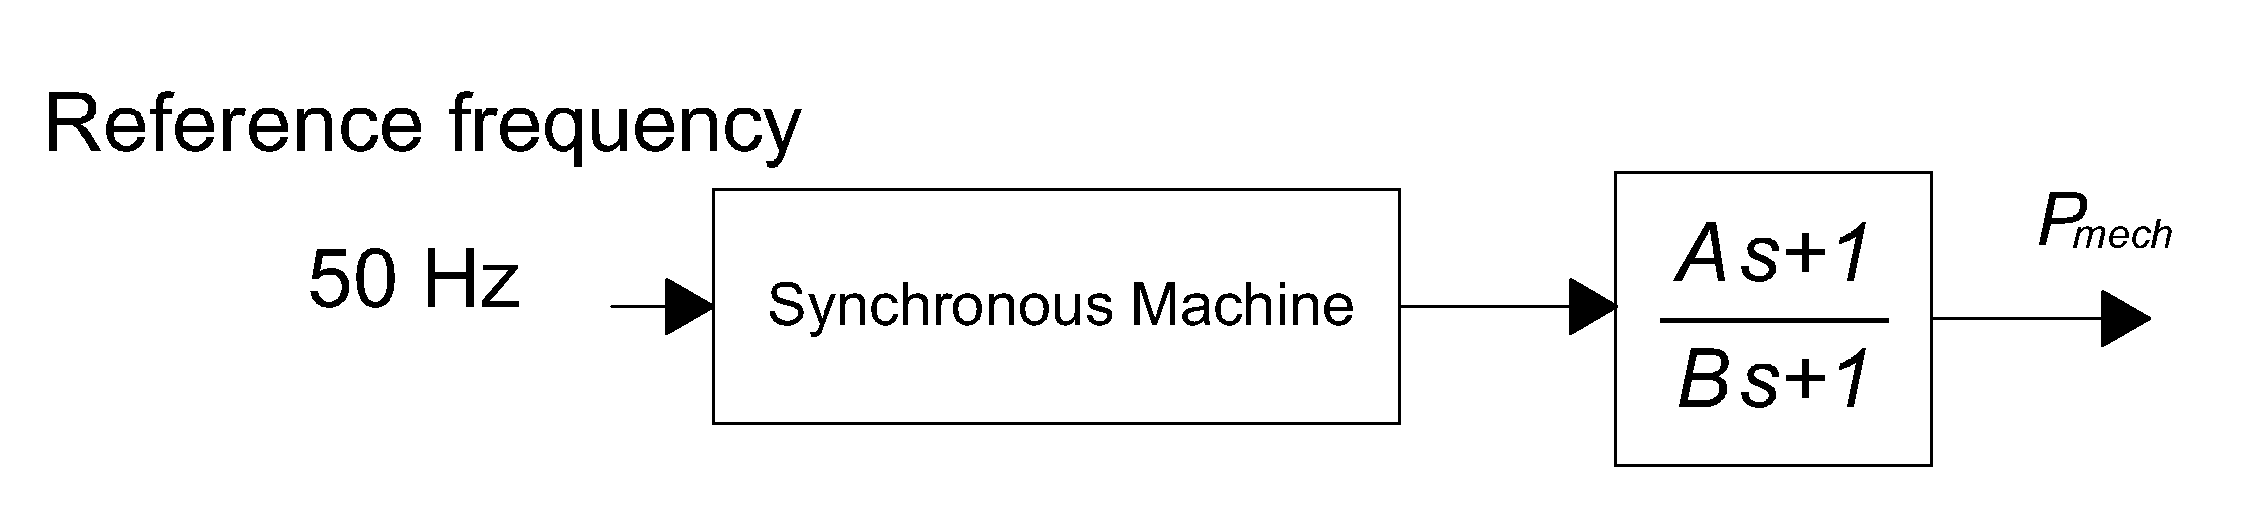
\includegraphics[width=0.5\textwidth]{/method/goveuro}
\caption{Governor representation for the large grid scale case. The synchronous machine block represents the governor model used in Section \ref{ssec:simpleieee}. The Control System Tuner App sets the constants A, B, C and D of the additional block in the model in order to have a step response with a rise time of $ \sim30s $ by establishing an overshoot of 2\% and a time constant of 8 seconds \cite{ogata1999ingenieria}.}
\label{fig:goveuro}
\end{figure}




\subsubsection{System Parameters}

When a power system of $ n $ number of synchronous machines is assumed; having each of them a capacity $ S $ in MVA, a nominal power $ P_{nom} $ in MW and
supposing that each machine operates at a de-load factor $ dl $ of $ P_{nom} $; with an acceleration constant equal to $ T_{nom} $ then the number of machines $ n $, for the load $ P_{syncload} $ served by synchronous machines is:
%Equation 3 12
%n=P_(load_sync)/(P_nom*dl)
\begin{equation}
n=\dfrac{P_{syncload}}{P_{nom}*dl}
\end{equation}
The time acceleration constant of the system $ T_{sys} $ can be obtained as follows:
\begin{align}
T_{sys} &=\dfrac{\sum_{i=1}^nP_i*T_i}{P_{LOAD}}\nonumber \\
&=\dfrac{nP_{nom}*T_i}{P_{LOAD}}\nonumber \\
&=\dfrac{P_{syncload}*T_{nom}}{P_{LOAD}*dl}\nonumber\\
&=\dfrac{Sync share*T_{nom}}{dl} \label{eq:tsyseuro}
\end{align}




In this sense the system's acceleration time constant can be calculated with a synchronous share of 100\%, resulting in $ T_{sys}=12.5s $ with values of $ T_{nom}=10s $ \cite{ENTSOE.2016, Anderson.2002}, and a de-load factor $ dl=0.8 $. Considering only the swing equation, it can be demonstrated that RoCoF and therefore the frequency response of the system is only dependent on the percentage of load imbalance and the system acceleration time constant.
From the definition of RoCoF as $ \frac{df}{dt}=\frac{\Delta P*f_0}{2*E_k} $ and $ T_{sys}=\frac{2*E_k}{P_{LOAD}} $ :

\begin{align}
\dfrac{df}{dt} &=\dfrac{\Delta P*f_0}{P_{LOAD}*T_{sys}} \nonumber\\
&=\dfrac{\Delta P_{pu}*f_0}{P_{LOAD}*T_{sys}}
\label{eq:dfdpeuro}
\end{align}
In Equation \eqref{eq:dfdpeuro} the value of $ \Delta P_{pu} $ is the normalized value of power imbalance having as base power the value of load $ P_{LOAD} $.